% This file was created with matplot2tikz v0.4.0.
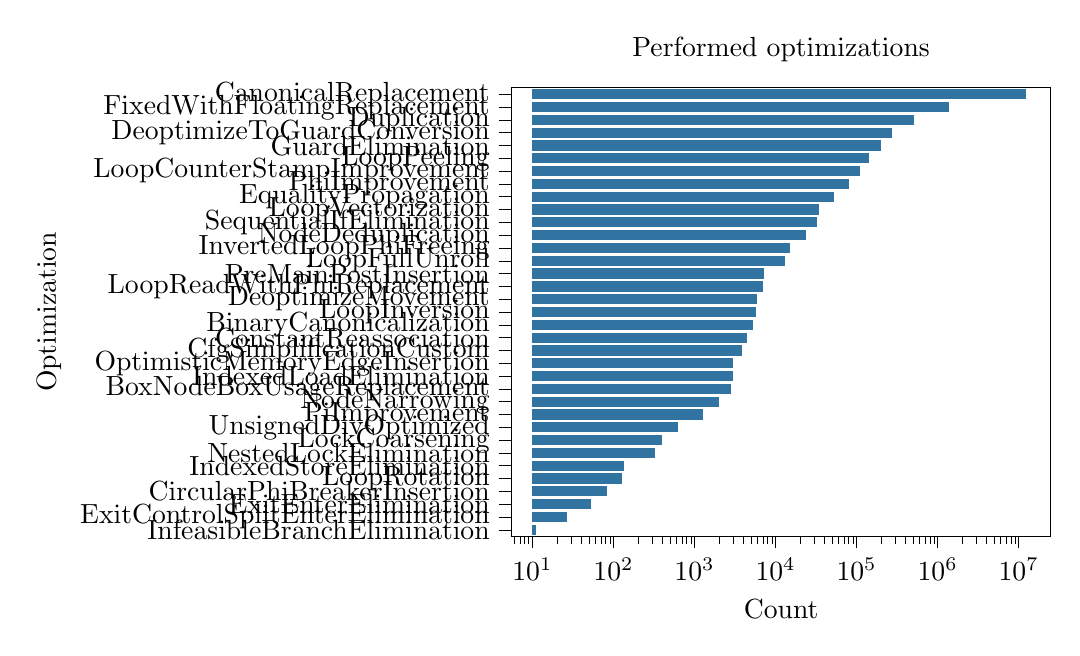
\begin{tikzpicture}

\definecolor{darkgray176}{RGB}{176,176,176}
\definecolor{darkslategray66}{RGB}{66,66,66}
\definecolor{steelblue49115161}{RGB}{49,115,161}

\begin{axis}[
log basis x={10},
tick align=outside,
tick pos=left,
title={Performed optimizations},
x grid style={darkgray176},
xlabel={Count},
xmin=5.47883750229848, xmax=25013948.8427072,
xmode=log,
xtick style={color=black},
y dir=reverse,
y grid style={darkgray176},
ylabel={Optimization},
ymin=-0.5, ymax=34.5,
ytick style={color=black},
ytick={0,1,2,3,4,5,6,7,8,9,10,11,12,13,14,15,16,17,18,19,20,21,22,23,24,25,26,27,28,29,30,31,32,33,34},
yticklabels={
  CanonicalReplacement,
  FixedWithFloatingReplacement,
  Duplication,
  DeoptimizeToGuardConversion,
  GuardElimination,
  LoopPeeling,
  LoopCounterStampImprovement,
  PhiImprovement,
  EqualityPropagation,
  LoopVectorization,
  SequentialIfElimination,
  NodeDeduplication,
  InvertedLoopPhiFreeing,
  LoopFullUnroll,
  PreMainPostInsertion,
  LoopReadWithPhiReplacement,
  DeoptimizeMovement,
  LoopInversion,
  BinaryCanonicalization,
  ConstantReassociation,
  CfgSimplificationCustom,
  OptimisticMemoryEdgeInsertion,
  IndexedLoadElimination,
  BoxNodeBoxUsageReplacement,
  NodeNarrowing,
  PiImprovement,
  UnsignedDivOptimized,
  LockCoarsening,
  NestedLockElimination,
  IndexedStoreElimination,
  LoopRotation,
  CircularPhiBreakerInsertion,
  ExitEnterElimination,
  ExitControlSplitEnterElimination,
  InfeasibleBranchElimination
}
]
\draw[draw=none,fill=steelblue49115161,line width=0.32pt] (axis cs:0,-0.4) rectangle (axis cs:12458851,0.4);\draw[draw=none,fill=steelblue49115161,line width=0.32pt] (axis cs:0,0.6) rectangle (axis cs:1383318,1.4);\draw[draw=none,fill=steelblue49115161,line width=0.32pt] (axis cs:0,1.6) rectangle (axis cs:508643,2.4);\draw[draw=none,fill=steelblue49115161,line width=0.32pt] (axis cs:0,2.6) rectangle (axis cs:269648,3.4);\draw[draw=none,fill=steelblue49115161,line width=0.32pt] (axis cs:0,3.6) rectangle (axis cs:198137,4.4);\draw[draw=none,fill=steelblue49115161,line width=0.32pt] (axis cs:0,4.6) rectangle (axis cs:143313,5.4);\draw[draw=none,fill=steelblue49115161,line width=0.32pt] (axis cs:0,5.6) rectangle (axis cs:109909,6.4);\draw[draw=none,fill=steelblue49115161,line width=0.32pt] (axis cs:0,6.6) rectangle (axis cs:81501,7.4);\draw[draw=none,fill=steelblue49115161,line width=0.32pt] (axis cs:0,7.6) rectangle (axis cs:52872,8.4);\draw[draw=none,fill=steelblue49115161,line width=0.32pt] (axis cs:0,8.6) rectangle (axis cs:34188,9.4);\draw[draw=none,fill=steelblue49115161,line width=0.32pt] (axis cs:0,9.6) rectangle (axis cs:32244,10.4);\draw[draw=none,fill=steelblue49115161,line width=0.32pt] (axis cs:0,10.6) rectangle (axis cs:23596,11.4);\draw[draw=none,fill=steelblue49115161,line width=0.32pt] (axis cs:0,11.6) rectangle (axis cs:15155,12.4);\draw[draw=none,fill=steelblue49115161,line width=0.32pt] (axis cs:0,12.6) rectangle (axis cs:13074,13.4);\draw[draw=none,fill=steelblue49115161,line width=0.32pt] (axis cs:0,13.6) rectangle (axis cs:7154,14.4);\draw[draw=none,fill=steelblue49115161,line width=0.32pt] (axis cs:0,14.6) rectangle (axis cs:7077,15.4);\draw[draw=none,fill=steelblue49115161,line width=0.32pt] (axis cs:0,15.6) rectangle (axis cs:5902,16.4);\draw[draw=none,fill=steelblue49115161,line width=0.32pt] (axis cs:0,16.6) rectangle (axis cs:5745,17.4);\draw[draw=none,fill=steelblue49115161,line width=0.32pt] (axis cs:0,17.6) rectangle (axis cs:5306,18.4);\draw[draw=none,fill=steelblue49115161,line width=0.32pt] (axis cs:0,18.6) rectangle (axis cs:4489,19.4);\draw[draw=none,fill=steelblue49115161,line width=0.32pt] (axis cs:0,19.6) rectangle (axis cs:3831,20.4);\draw[draw=none,fill=steelblue49115161,line width=0.32pt] (axis cs:0,20.6) rectangle (axis cs:3021,21.4);\draw[draw=none,fill=steelblue49115161,line width=0.32pt] (axis cs:0,21.6) rectangle (axis cs:2957,22.4);\draw[draw=none,fill=steelblue49115161,line width=0.32pt] (axis cs:0,22.6) rectangle (axis cs:2851,23.4);\draw[draw=none,fill=steelblue49115161,line width=0.32pt] (axis cs:0,23.6) rectangle (axis cs:2014,24.4);\draw[draw=none,fill=steelblue49115161,line width=0.32pt] (axis cs:0,24.6) rectangle (axis cs:1264,25.4);\draw[draw=none,fill=steelblue49115161,line width=0.32pt] (axis cs:0,25.6) rectangle (axis cs:634,26.4);\draw[draw=none,fill=steelblue49115161,line width=0.32pt] (axis cs:0,26.6) rectangle (axis cs:401,27.4);\draw[draw=none,fill=steelblue49115161,line width=0.32pt] (axis cs:0,27.6) rectangle (axis cs:323,28.4);\draw[draw=none,fill=steelblue49115161,line width=0.32pt] (axis cs:0,28.6) rectangle (axis cs:136,29.4);\draw[draw=none,fill=steelblue49115161,line width=0.32pt] (axis cs:0,29.6) rectangle (axis cs:129,30.4);\draw[draw=none,fill=steelblue49115161,line width=0.32pt] (axis cs:0,30.6) rectangle (axis cs:84,31.4);\draw[draw=none,fill=steelblue49115161,line width=0.32pt] (axis cs:0,31.6) rectangle (axis cs:53,32.4);\draw[draw=none,fill=steelblue49115161,line width=0.32pt] (axis cs:0,32.6) rectangle (axis cs:27,33.4);\draw[draw=none,fill=steelblue49115161,line width=0.32pt] (axis cs:0,33.6) rectangle (axis cs:11,34.4);\addplot [line width=0.72pt, darkslategray66]
table {%
nan 0
nan 0
};
\addplot [line width=0.72pt, darkslategray66]
table {%
nan 1
nan 1
};
\addplot [line width=0.72pt, darkslategray66]
table {%
nan 2
nan 2
};
\addplot [line width=0.72pt, darkslategray66]
table {%
nan 3
nan 3
};
\addplot [line width=0.72pt, darkslategray66]
table {%
nan 4
nan 4
};
\addplot [line width=0.72pt, darkslategray66]
table {%
nan 5
nan 5
};
\addplot [line width=0.72pt, darkslategray66]
table {%
nan 6
nan 6
};
\addplot [line width=0.72pt, darkslategray66]
table {%
nan 7
nan 7
};
\addplot [line width=0.72pt, darkslategray66]
table {%
nan 8
nan 8
};
\addplot [line width=0.72pt, darkslategray66]
table {%
nan 9
nan 9
};
\addplot [line width=0.72pt, darkslategray66]
table {%
nan 10
nan 10
};
\addplot [line width=0.72pt, darkslategray66]
table {%
nan 11
nan 11
};
\addplot [line width=0.72pt, darkslategray66]
table {%
nan 12
nan 12
};
\addplot [line width=0.72pt, darkslategray66]
table {%
nan 13
nan 13
};
\addplot [line width=0.72pt, darkslategray66]
table {%
nan 14
nan 14
};
\addplot [line width=0.72pt, darkslategray66]
table {%
nan 15
nan 15
};
\addplot [line width=0.72pt, darkslategray66]
table {%
nan 16
nan 16
};
\addplot [line width=0.72pt, darkslategray66]
table {%
nan 17
nan 17
};
\addplot [line width=0.72pt, darkslategray66]
table {%
nan 18
nan 18
};
\addplot [line width=0.72pt, darkslategray66]
table {%
nan 19
nan 19
};
\addplot [line width=0.72pt, darkslategray66]
table {%
nan 20
nan 20
};
\addplot [line width=0.72pt, darkslategray66]
table {%
nan 21
nan 21
};
\addplot [line width=0.72pt, darkslategray66]
table {%
nan 22
nan 22
};
\addplot [line width=0.72pt, darkslategray66]
table {%
nan 23
nan 23
};
\addplot [line width=0.72pt, darkslategray66]
table {%
nan 24
nan 24
};
\addplot [line width=0.72pt, darkslategray66]
table {%
nan 25
nan 25
};
\addplot [line width=0.72pt, darkslategray66]
table {%
nan 26
nan 26
};
\addplot [line width=0.72pt, darkslategray66]
table {%
nan 27
nan 27
};
\addplot [line width=0.72pt, darkslategray66]
table {%
nan 28
nan 28
};
\addplot [line width=0.72pt, darkslategray66]
table {%
nan 29
nan 29
};
\addplot [line width=0.72pt, darkslategray66]
table {%
nan 30
nan 30
};
\addplot [line width=0.72pt, darkslategray66]
table {%
nan 31
nan 31
};
\addplot [line width=0.72pt, darkslategray66]
table {%
nan 32
nan 32
};
\addplot [line width=0.72pt, darkslategray66]
table {%
nan 33
nan 33
};
\addplot [line width=0.72pt, darkslategray66]
table {%
nan 34
nan 34
};
\end{axis}

\end{tikzpicture}
